\chapter{Introduction}
In this thesis the initial task was to learn how street networks and buildings can be described as grammar for later analysis and regeneration. There exist many different approaches like Shape Grammars \ref{sec:shape_grammar} (building faces generation), L-Systems \ref{sec:L-Systems} (plants growing), Space Syntax \ref{sec:space_syntax} and many others. Because the application \acrshort{acr:CPlan} \ref{CPlan} did not provide the ability to use grammars and our customer preferred a graph based approach all later described algorithms are based on unidirectional graphs.

The \gls{iA} provided computational planning tools named \acrshort{acr:CPlan} \ref{CPlan}. To become acquainted with the application and to provide a way to create chromosomes for the existing genetic algorithms from street networks a tree generation algorithm was developed.

Selecting interesting areas from different cities and recombining them into a new one would allow a fast creation of new cities. To reach this goal many steps are necessary. First of all the cities must be separated into reasonable parts based on vertex position or edge length. The approach of this thesis is to use clustering algorithms from the field of machine learning. Useful cluster areas can then be selected by comparing different measured values like the variance of the street length or the median block length.

For this thesis the centroid-based \ref{sec:K-Means} clustering algorithm K-Means was implemented and tested. To improve the results --- so that clusters are guaranteed to be connected subgraphs --- \gls{APSP} algorithms were used \ref{sec:K-Means_shortest_path}.

Another approach were the hierarchical clustering algorithms \ref{sec:hierarchicalClustering} where different reduction formula exist. First the Single-Linkage formula was realised. Unfortunately only one cluster in the centre with many small clusters at the surrounding was created.

%Quickfix
\newpage

Then the reduction formulae \gls{UPGMA} and \gls{WPGMA} were implemented and tested \ref{sec:UPGMAandWPGMA}. These approaches created way better clusters but the cluster sizes could sometimes vary widely in size in a single clustering result.

More equally sized clusters then where achieved by modifying the output \ref{sec:concept_cluster_sizes}. Instead of splitting the hierarchy in the order it was created, always the cluster with the most notes was split. As a result the areas where more equally sized which is often preferred in city clustering. The result can be viewed in figure  \ref{fig:cluster_with_mod_sizes}.

\begin{figure}[ht]
    \centering
    \begin{mdframed}[style=mdthight, userdefinedwidth=0.4\linewidth, align=center]
        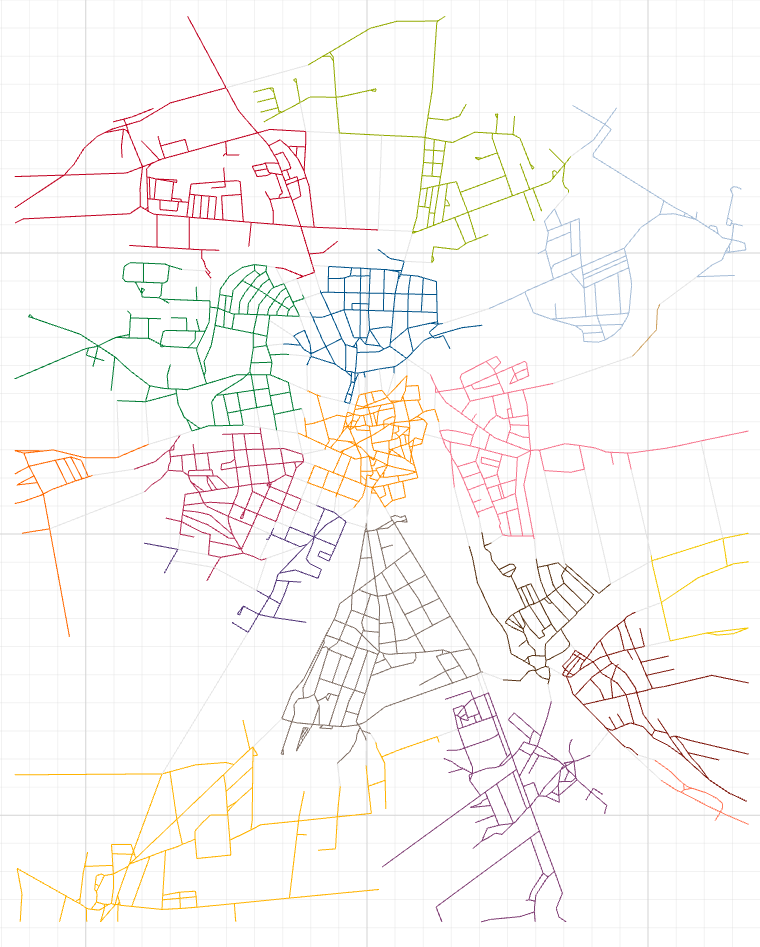
\includegraphics[width=\linewidth]{modified_cluster_size.png}
    \end{mdframed}
    \caption{Clusters with modified size}
    \label{fig:cluster_with_mod_sizes}
\end{figure}

During tests of initial implementations of the hierarchical clustering methods with big cities they caused high memory usage \ref{sec:concept_memory_usage}. To reduce the memory footprint, optimisations were applied and specialized data structures were realised.

The created clusters were then measured \ref{sec:measurements-cluster-analysis} and compared based on the suggestions \ref{sec:clusterRating} provided by the ETH-Zurich. Additionally the results can now be exported into a JSON-File for further use.

To recombine the separated areas/districts to a new city another project at ETH-Zurich is currently working on a regrow algorithm \ref{sec:future_work}. 